\documentclass{article}

\usepackage[english]{babel}
\usepackage[utf8]{inputenc}
\usepackage{amsmath,amssymb}
\usepackage{parskip}
\usepackage{graphicx}
\usepackage{listings}
\usepackage{float}
\usepackage{subfig}

\lstset{
    numbers=left, 
    numberstyle= \tiny, 
    keywordstyle= \color{ blue!70},
    commentstyle= \color{red!50!green!50!blue!50}, 
    frame=shadowbox, % 阴影效果
    rulesepcolor= \color{ red!20!green!20!blue!20} ,
    escapeinside=``, % 英文分号中可写入中文
    xleftmargin=2em,xrightmargin=2em, aboveskip=1em,
    framexleftmargin=2em,
    language = R,
    breaklines = true
} 

% Margins
\usepackage[top=2.5cm, left=3cm, right=3cm, bottom=4.0cm]{geometry}
% Colour table cells
\usepackage[table]{xcolor}

% Get larger line spacing in table
\newcommand{\tablespace}{\\[1.25mm]}
\newcommand\Tstrut{\rule{0pt}{2.6ex}}         % = `top' strut
\newcommand\tstrut{\rule{0pt}{2.0ex}}         % = `top' strut
\newcommand\Bstrut{\rule[-0.9ex]{0pt}{0pt}}   % = `bottom' strut

%%%%%%%%%%%%%%%%%
%     Title     %
%%%%%%%%%%%%%%%%%
\title{CSCI946 Assignment}
\author{Yao Xiao \\ SID 2019180015}
\date{\today}

\begin{document}
\maketitle

%%%%%%%%%%%%%%%%%
%   Problem 1   %
%%%%%%%%%%%%%%%%%
\section{Problem 1}
\begin{lstlisting}
library(arules)
library(arulesViz)

data("Groceries")

class(Groceries)
inspect(head(Groceries, 2))

# Get itemsets of length 1
itemsets <- apriori(Groceries, parameter = list(minlen=1,maxlen=10,support=0.02
,target="frequent itemsets"))

summary(itemsets)

itemsets <- apriori(Groceries, parameter = list(minlen=2,maxlen=10,support=0.02
,target="frequent itemsets"))

summary(itemsets)

itemsets <- apriori(Groceries, parameter = list(minlen=4,maxlen=4,support=0.02
,target="frequent itemsets"))

summary(itemsets)

# lists top 10
inspect(head(sort(itemsets,by="support"),10))
\end{lstlisting}

\begin{figure}[H]
  \centering
  \caption{Outputs of the Apriori algorithm}
  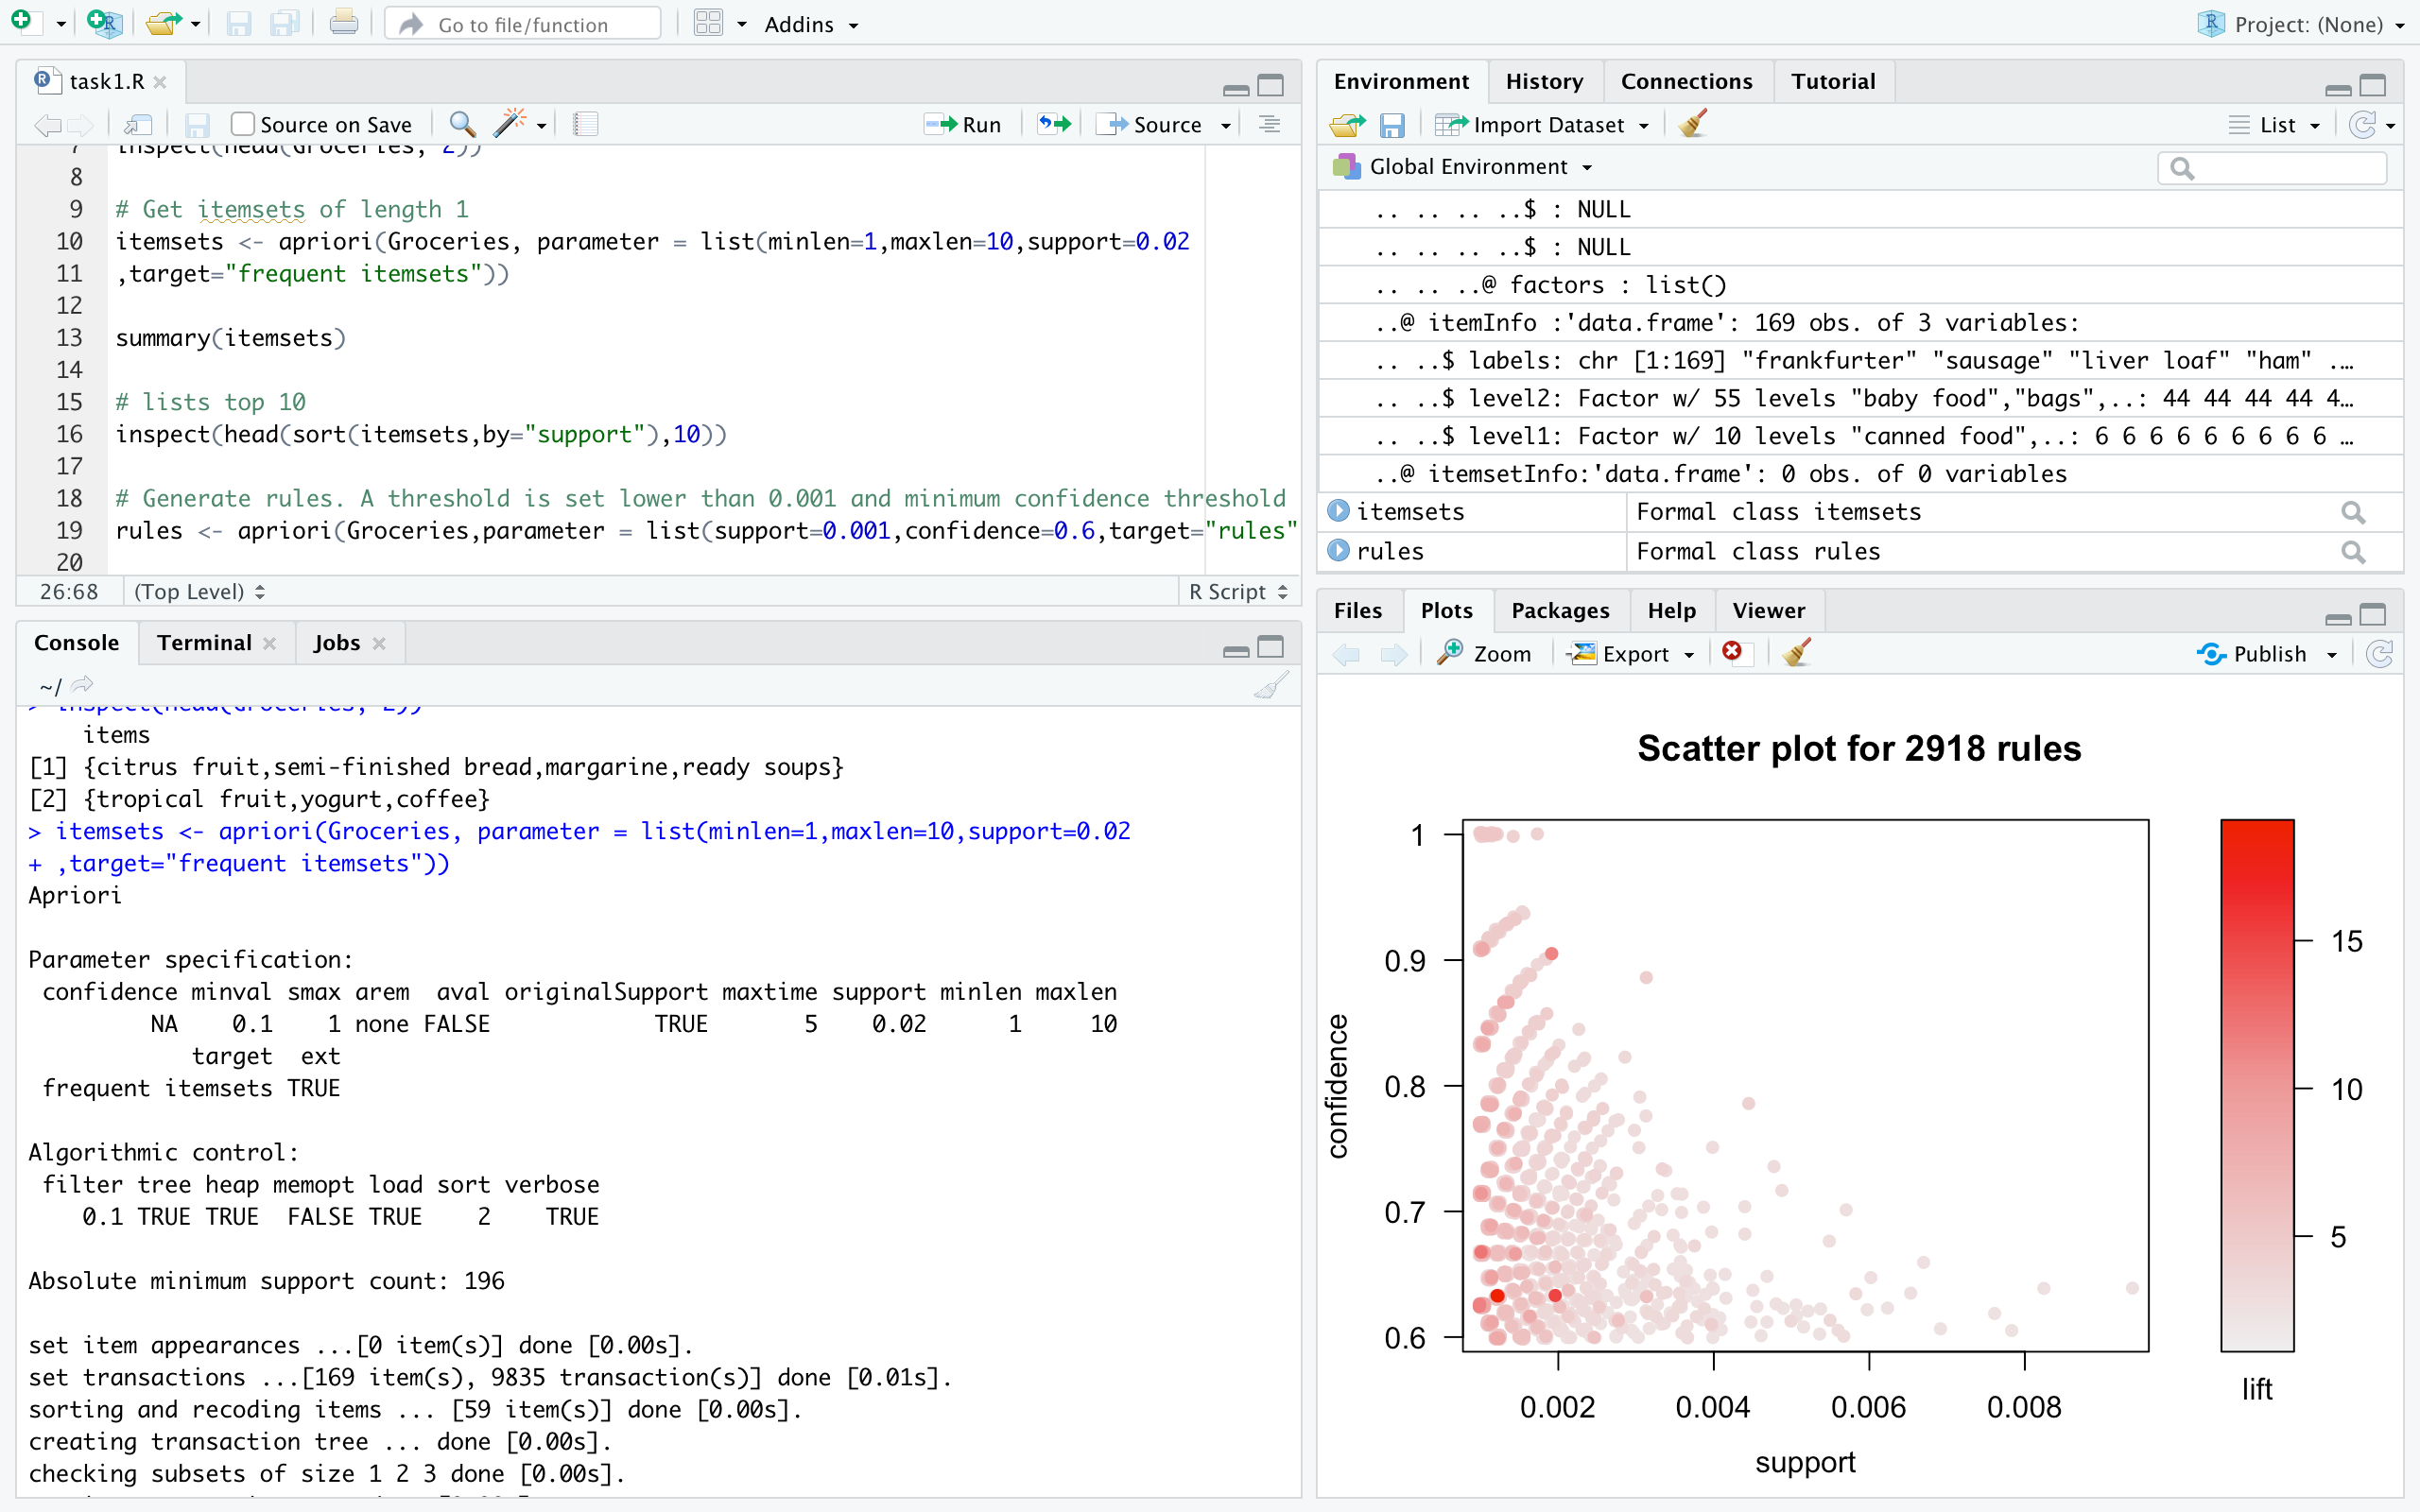
\includegraphics[width=0.6\textwidth]{Fig0}
\end{figure}

\section{Problem 2}
\begin{lstlisting}
library(arules)
library(arulesViz)

data("Groceries")

class(Groceries)
inspect(head(Groceries, 2))

# Get itemsets of length 1
itemsets <- apriori(Groceries, parameter = list(minlen=1,maxlen=10,support=0.02
,target="frequent itemsets"))

summary(itemsets)

itemsets <- apriori(Groceries, parameter = list(minlen=2,maxlen=10,support=0.02
,target="frequent itemsets"))

summary(itemsets)

itemsets <- apriori(Groceries, parameter = list(minlen=4,maxlen=4,support=0.02
,target="frequent itemsets"))

summary(itemsets)

# lists top 10
inspect(head(sort(itemsets,by="support"),10))

# generate rules. A threshold is set lower than 0.001 and minimum confidence threshold is set to 0.6.
rules <- apriori(Groceries,parameter = list(support=0.001,confidence=0.6,target="rules"))

summary(rules)

plot(rules)       

# compute the 1/Support(Y) is slope
slope <- sort(round(rules@quality$lift/rules@quality$confidence,2))

# display the number of times each slope appears
unlist(lapply(split(slope,f=slope),length))

inspect(head(sort(rules,by="lift"),10))

confidentRules<-rules[quality(rules)$confidence>0.9]
confidentRules

# plot a matrix-based visualization of the LHS v RHS of rules.
plot(confidentRules,method="matrix",measure=c("lift","confidence"),control=list(reorder="none"))

# visualize the top 5 rules with the highest lift
highLiftRules<-head(sort(rules,by="lift"),5)
plot(highLiftRules,method="graph",control=list(type="items"))
\end{lstlisting}

\begin{figure}[H]
  \centering
  \caption{Scatter plot of the generated rules}
  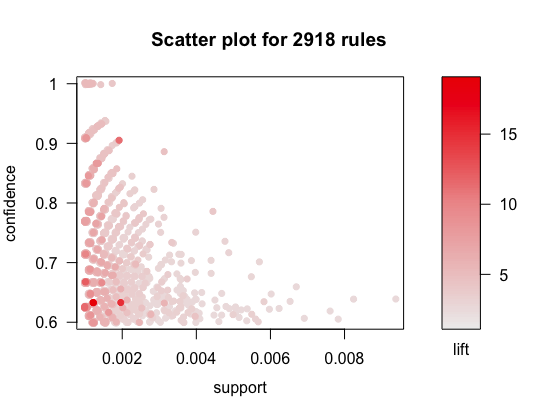
\includegraphics[width=0.6\textwidth]{Fig1}
\end{figure}

\begin{figure}[H]
  \centering
  \caption{Scatter matrix}
  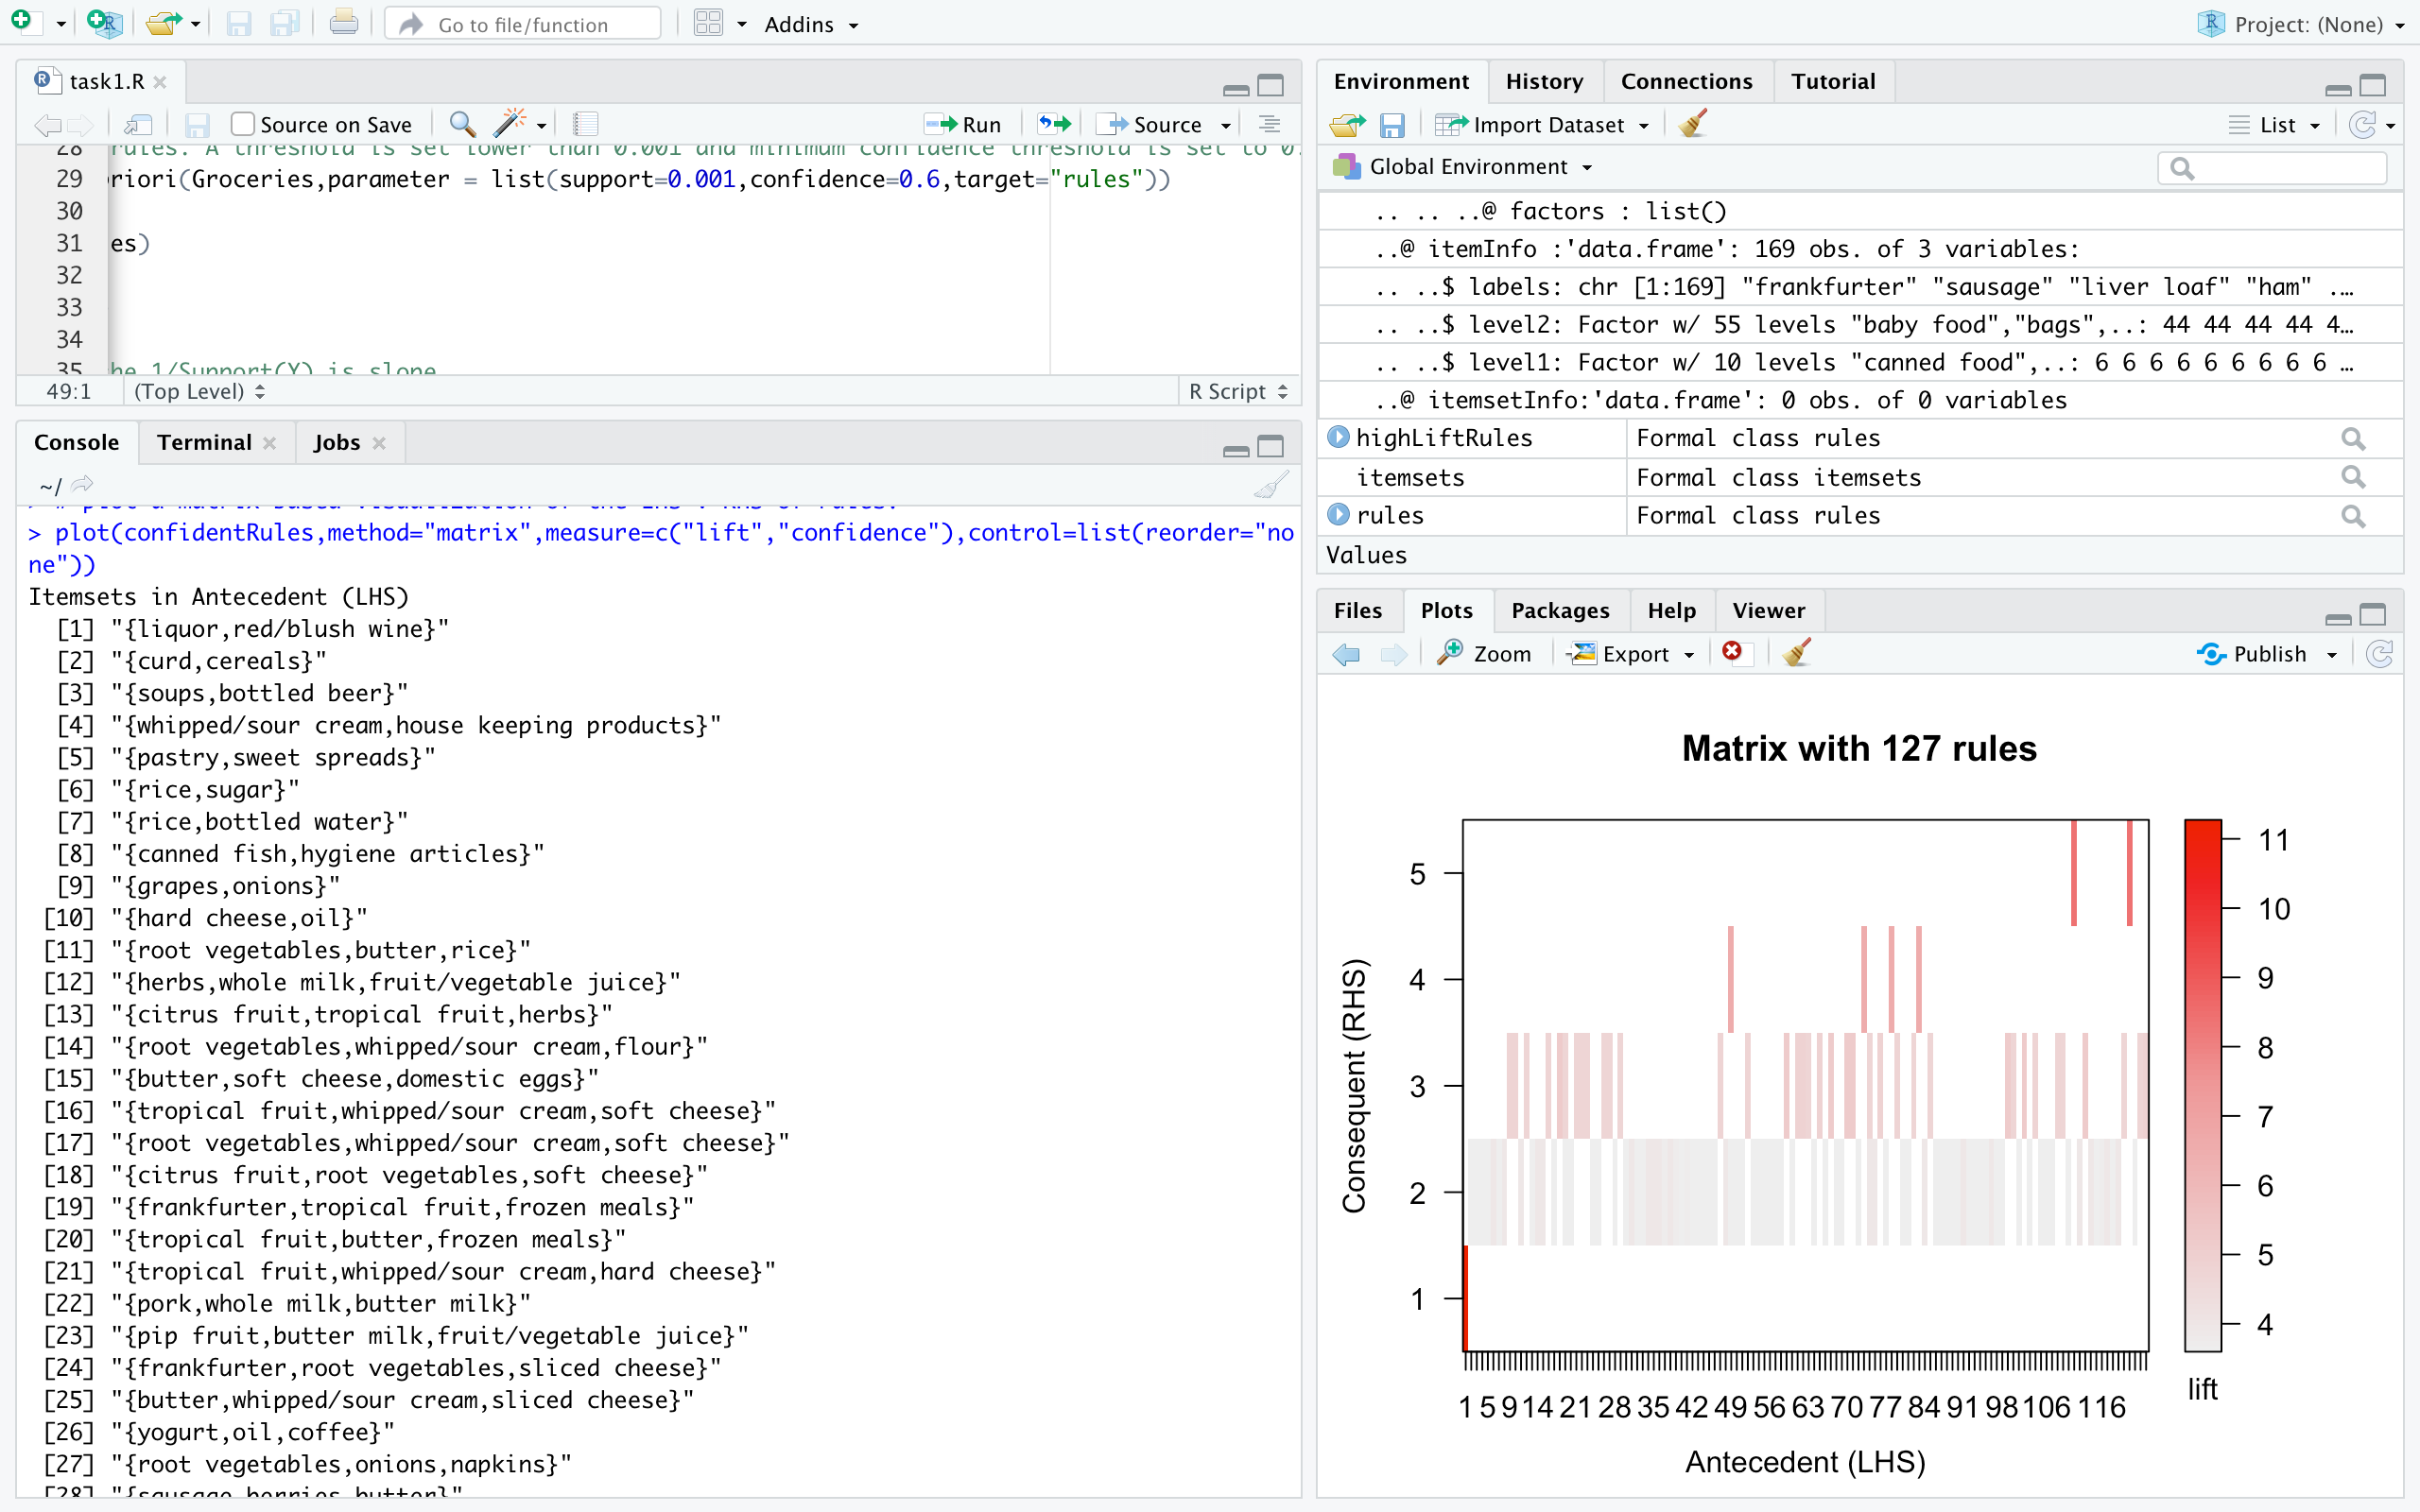
\includegraphics[width=0.6\textwidth]{Fig4}
\end{figure}

\begin{figure}[H]
  \centering
  \caption{Matrix-based visualization of the LHS and RHS}
  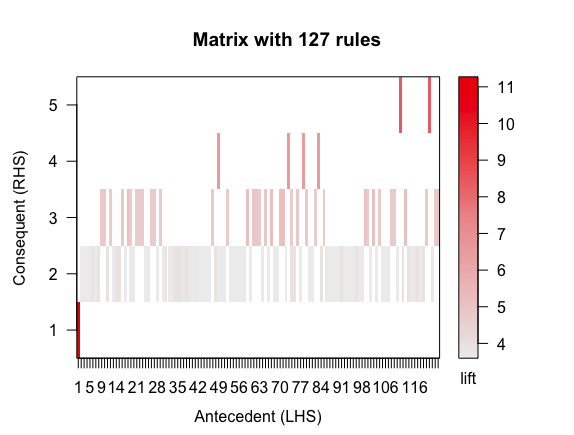
\includegraphics[width=0.6\textwidth]{Fig2}
\end{figure}

\begin{figure}[H]
  \centering
  \caption{Graph visualization of the top five rules}
  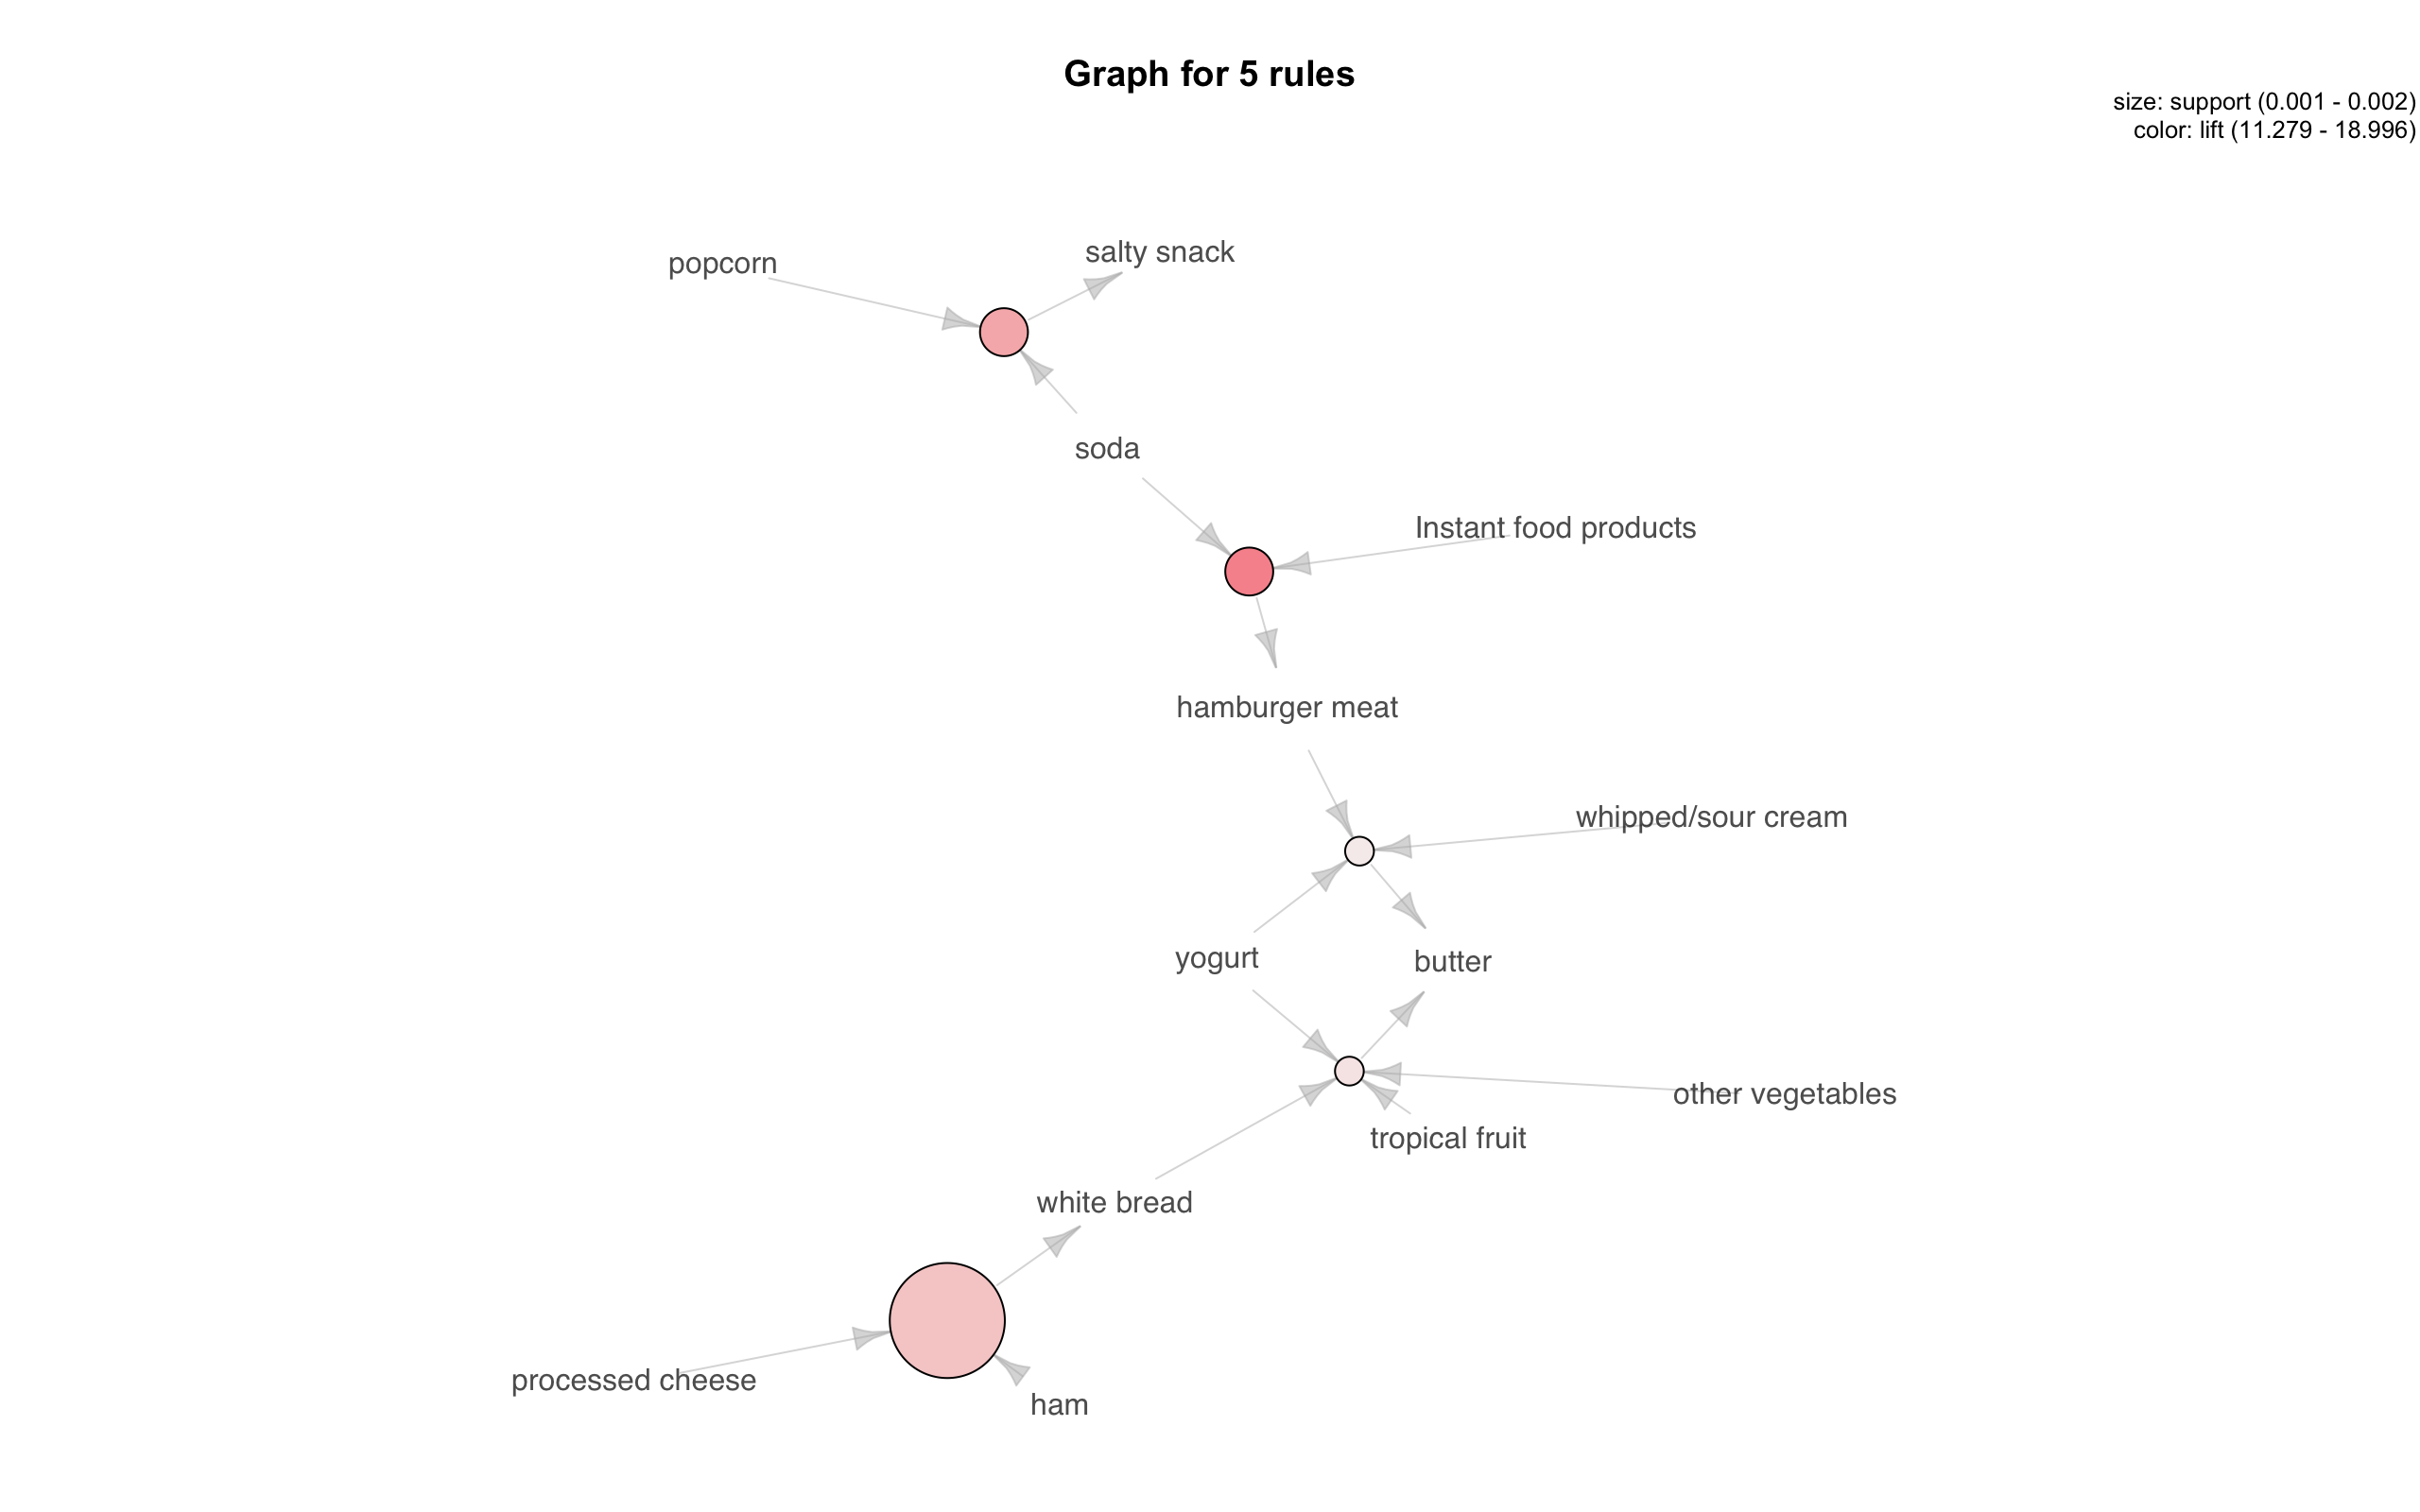
\includegraphics[width=0.6\textwidth]{Fig3}
\end{figure}


\end{document}

